\chapter{Introduction}
\label{chapter1}

Robots are emerging from controlled factories and
laboratories into our homes, workplaces, roads, and public airspaces.
Alongside their transition into these unstructured and transient environments
comes their need to be able to explore, characterize, and catalog their surroundings.
Mobile robot autonomy is generally accomplished by referring to a map - a 2D or 3D
probabilistic representation of the locations of obstacles in the robot's workspace.
With access to a map, robots can localize to determine their position, plan collision-free
trajectories to goals, locate objects for interaction, and make decisions by
reasoning about the geometry and dynamics of the world. Given that a robot's map
is of critical importance for most autonomy tasks, robots that find
themselves initialized without a priori access to a map should be capable of
autonomously, efficiently, and intelligently creating one.

The exercise of choosing and executing actions that lead a robot to learn more about its own
map is known as \textit{active perception} or \textit{exploration}, and
is the central topic of this thesis. Active perception has previously been studied with a
multitude of sensor models, environment representations, and robot dynamics
models. The active perception task itself can be dissected into two
components~\cite{shen20113d}:

\begin{enumerate}[leftmargin=3.2cm]
  \item[\bf component 1:] Identifying and ranking actions that the robot can
    take to spatially extend or reduce uncertainty in its map
  \item[\bf component 2:] Autonomously navigating according to the most informative
    action, while simultaneously localizing to the map and updating it with incoming sensor
    measurements
\end{enumerate}

A motivating example is depicted in Fig.~\ref{fig:motivation}, where a household
service robot is initialized in an unknown environment. Prior to accomplishing
tasks that a human might ask it to perform, the robot must learn its
surroundings and build a map of the house. Ideally this phase of
initialization would be fast, as it is a prerequisite to the main functionality
of the robot, and also might be required when furniture is moved or
household objects are displaced. Where should the robot travel to observe the
most of the environment in the shortest amount of time? Virtually any autonomous robot
operating in an unknown environment will require a map-building
initialization phase, welcoming strategies that enable high-speed and intelligent
exploration.

\begin{figure}[t]
  \centering
  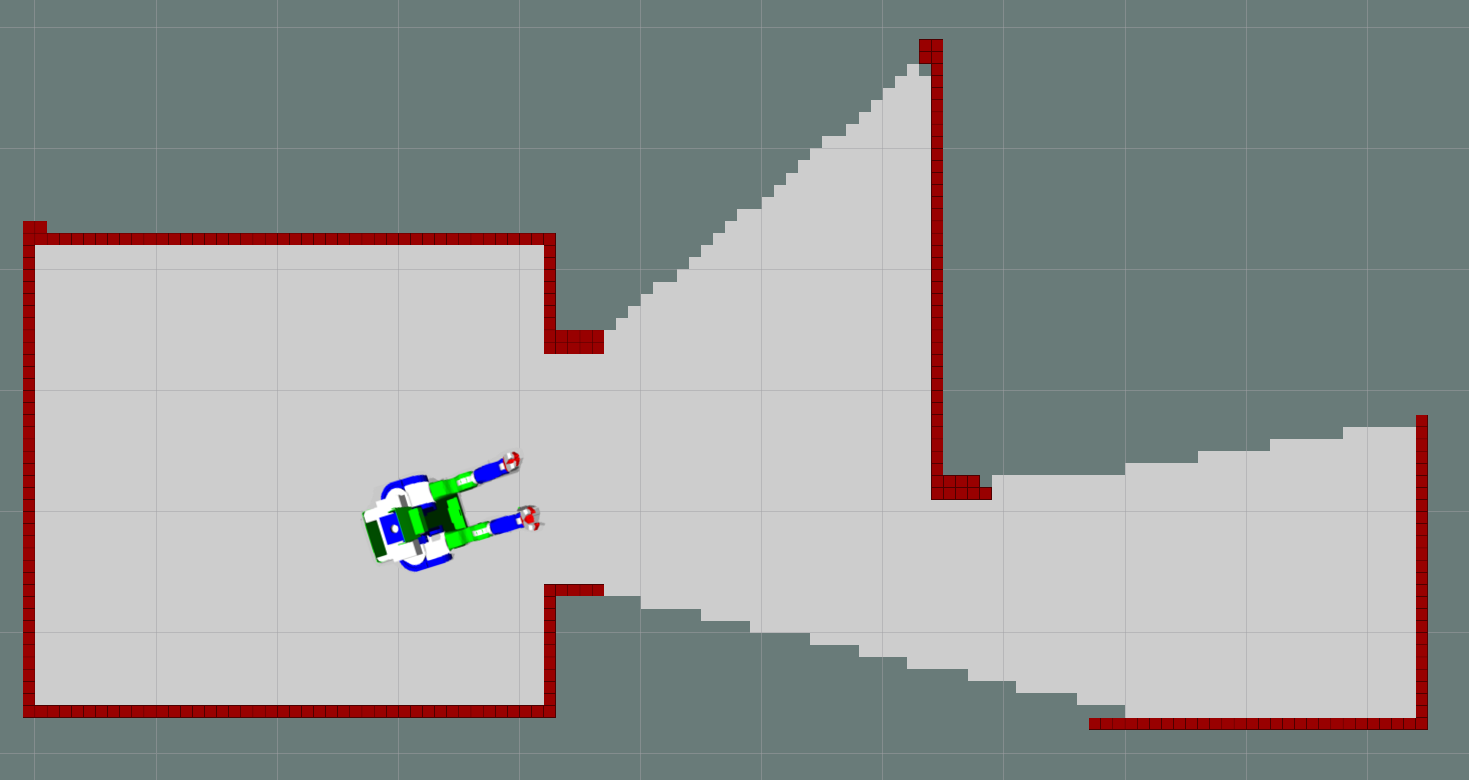
\includegraphics[width=0.6\textwidth]{explore.png}
  \caption[A household service robot must explore its unknown environment.]{A
    household service robot awakens in an unknown environment. Prior to
  accomplishing its main functionalities, it will require a map of its surroundings.
What sequence of actions should it take to minimize the time it spends
exploring? \label{fig:motivation}}
\end{figure}

This thesis explores one method for making {\bf component 1} more efficient,
thereby allowing an exploring robot to either consider more future actions in
the same amount of time, or the same amount of actions in a shorter amount of
time. By considering more actions, the robot has a higher likelihood of
finding one that is informative. By considering actions in a shorter amount of
time, the robot is able to alot more computational resources to other tasks,
such as planning, mapping, and control, thereby allowing it to achieve {\bf
component 2} at higher speeds. Combined, these implications allow a robot to explore an unknown
environment more efficiently than it would otherwise be able to.

%This thesis develops methods for increasing the velocity at which a robot can
%accomplish {\bf component 2} of the active perception task by reducing the
%computational cost of performing {\bf component 1}. Increasing a robot's
%velocity while navigating to informative locations will allow it to explore more
%efficiently by learning a larger map in a given amount of time. However,
%na\"{i}vely increasing velocity is not enough to avoid collisions or guarantee
%efficient exploration behavior; the robot's maximum safe velocity is intricately
%tied to other parametrs, such as planning frequency, map update frequency, and number
%of planned future actions. Higher navigation velocities demand higher values for
%all of these parameters, which share finite computational resources.

%Achieving
%high speed exploration requires identifying computational bottlenecks and increasing and balancing these parameters


%Reducing the computational cost of {\bf component 1}
%will result in the robot being able to consider more possible future actions
%that it can take per unit time, giving it a higher likelihood of choosing an
%action that guides it to informative locations.
%Evaluating the informativeness
%of future actions has a computational cost that is a function of the resolution
%of the robot's map. Map compression is therefore proposed as a means of

%This thesis develops methods for increasing the efficiency of at which a robot is able
%to explore an unknown environment.

%Several aspects of the exploration task
%can be improved to result in the robot learning a larger map in a shorter
%amount of timea

%This thesis puts forth the claim that the speed-limiting factor for exploration is {\bf
%component 1},

%and develops methods for increasing its computational efficiency. State-of-the-art approaches
%in exploration employ techniques that compute control actions by analyzing information-theoretic
%metrics on the robot's map~\cite{bourgault2002information,kollar2008efficient,charrow2015icra,julian2013mutual}.
%Information-theoretic metrics generally have a fixed computational cost that is a
%function of the robot's sensor model. As a robot moves faster through an
%environment, it must evaluate the same metric on a fixed-size set of planned
%future actions, but in a shorter amount of time.

Map compression (decreasing a map's resolution) is proposed as a means of reducing the computational cost of
{\bf component 1}. This thesis will examine the ties between a map's resolution
and the expected informativeness of planned actions, and use this relationship to formulate
methods for optimally compressing a robot's map based on the local environment
and incoming sensor measurements. These considerations ultimately allow an
exploring robot to navigate more quickly and select more
informative actions for navigation.

%This thesis specifically considers the effects of environment representation on
%autonomous exploration behaviors, and introduces novel extensions to the active perception
%task that adaptively modify the environment representation in response to
%the robot's incoming sensor measurements and current map. The interplay between the robot's
%environment representation and exploration behaviors is investigated. First, a theory of
%information-theoretic map compression is developed. The map compression
%formulation is exercised to examine the information lost about a sensor
%measurement when compressing a map. Optimizing sensor information loss against
%map compression allows the robot to choose a resolution with which to
%represent its environment that maximizes the efficiency of exploration.
%The information lost through map compression can also be used to analyze the
%complexity and obstacle density of an environment. This second loss metric
%is added to the exploration reward function, allowing an autonomously exploring
%robot to choose trajectories that are both informative and safe for high-speed
%navigation.

%The proposed active perception extensions enable two new capabilities:

%\begin{enumerate}
%  \item Compressing the robot's map, when possible, increases the
%    efficiency of computing information-theoretic reward by orders of magnitude, thereby
%    enabling faster planning and navigation during exploration
%  \item Analyzing the loss in informativeness of sensor measurements when
%    compressing the map enables the robot to choose trajectories are both safe
%    (avoiding obstacle-dense regions)
%    and informative (maximizing an information-based reward).
%\end{enumerate}


\section{Previous Work}

Prior approaches to mobile robot active perception fall into two
broad categories: \textit{geometric} approaches that reason about the locations and
presence of obstacles and free space in the robot's
map~\cite{acar2002sensor,chan1993line,wang2007view,
burgard2000collaborative,taylor1993exploration,yamauchi1997frontier}, and
\textit{information-theoretic} approaches that treat the map as
a multivariate random variable and choose actions that will maximally reduce its
uncertainty~\cite{amigoni2010information,bourgault2002information,charrow2015icra,
julian2013mutual,feder1999adaptive}. Both categories of approaches solve {\bf
component 1} of active perception, and assume that a planner and Simultaneous
Localization and Mapping (SLAM) framework are available to accomplish {\bf
component 2}.

\subsection{Geometric Exploration Strategies}

Many successful geometric exploration approaches build upon the seminal work of
Yamauchi~\cite{yamauchi1997frontier}, guiding the robot to \textit{frontiers} - regions on the boundary
between free and unexplored space in the map (Fig.~\ref{fig:frontiers}).
Since multiple frontiers often exist simultaneously in a partially explored map, a
variety of heuristics and spatial metrics can be used to decide which frontier to
travel towards~\cite{lavalle2006planning}. For example, an agent may decide to
visit the frontier whose path through the configuration space from the agent's current
position has minimum length, or requires minimal time or energy input to
traverse. Similarly, an agent may decide to only plan paths to locations
from which frontiers can be observed by its onboard sensors.

\begin{figure}[t]
  \centering
  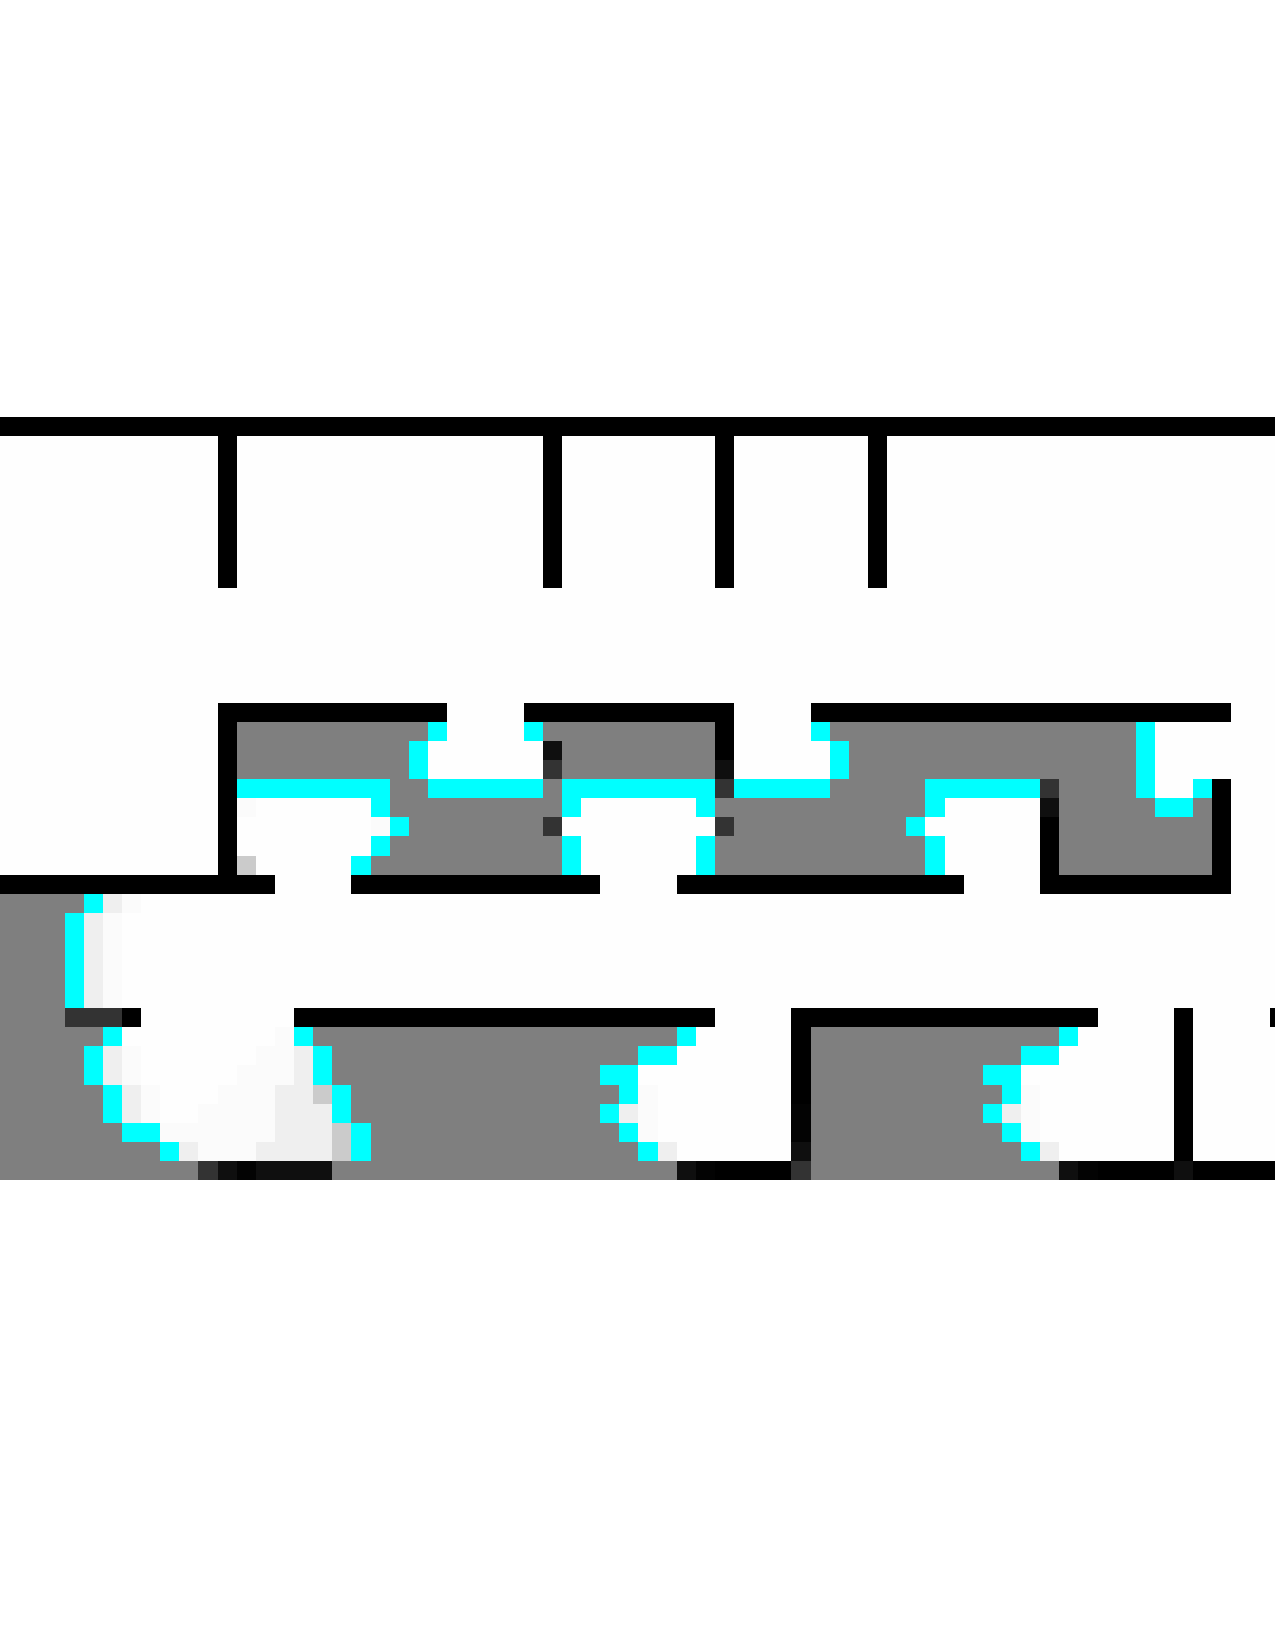
\includegraphics[trim=0cm 0.4cm 0.1cm 0.1cm, clip, width=0.8\textwidth]{frontiers.pdf}
  \caption[Frontiers in a partially explored map.]{A partially explored map with frontiers between free and unknown
  space highlighted in blue.\label{fig:frontiers}}
\end{figure}

While effective in 2D environments, frontier exploration algorithms have
several restrictive qualities. First, the na\"{i}ve extension of frontier exploration
from 2D to 3D maps poses a non-trivial challenge; as the
dimensionality of the workspace increases, frontiers are distributed more
densely throughout the environment due to occlusions, sensing resolution, and
field-of-view, resulting in poor exploration performance~\cite{shen20113d}.
Second, planning a path to a frontier does not imply that the path
itself will be information-rich. Trajectory optimization techniques that
consider information acquired by the robot's sensors along a planned path can be used
as extensions to improve exploration performance~\cite{sim2004online,kollar2008trajectory}.
Finally, although the robot is guaranteed to learn new information upon reaching a
frontier, the amount of information learned is dependent on the
robot's sensor model, which is not considered when identifying frontiers.
It may therefore be more efficient to visit a frontier that is
suboptimal according to heuristics such as path length if the robot's sensors
will provide more information from that location
(Fig.~\ref{fig:sensor_frontier}).
This limitation was first overcome by evaluating the informativeness of simulated
sensor measurements taken from frontier locations~\cite{gonzalez2002navigation}, and was the
original motivation for developing a category of information-theoretic exploration strategies.

\begin{figure}[t]
  \centering
  \centering
  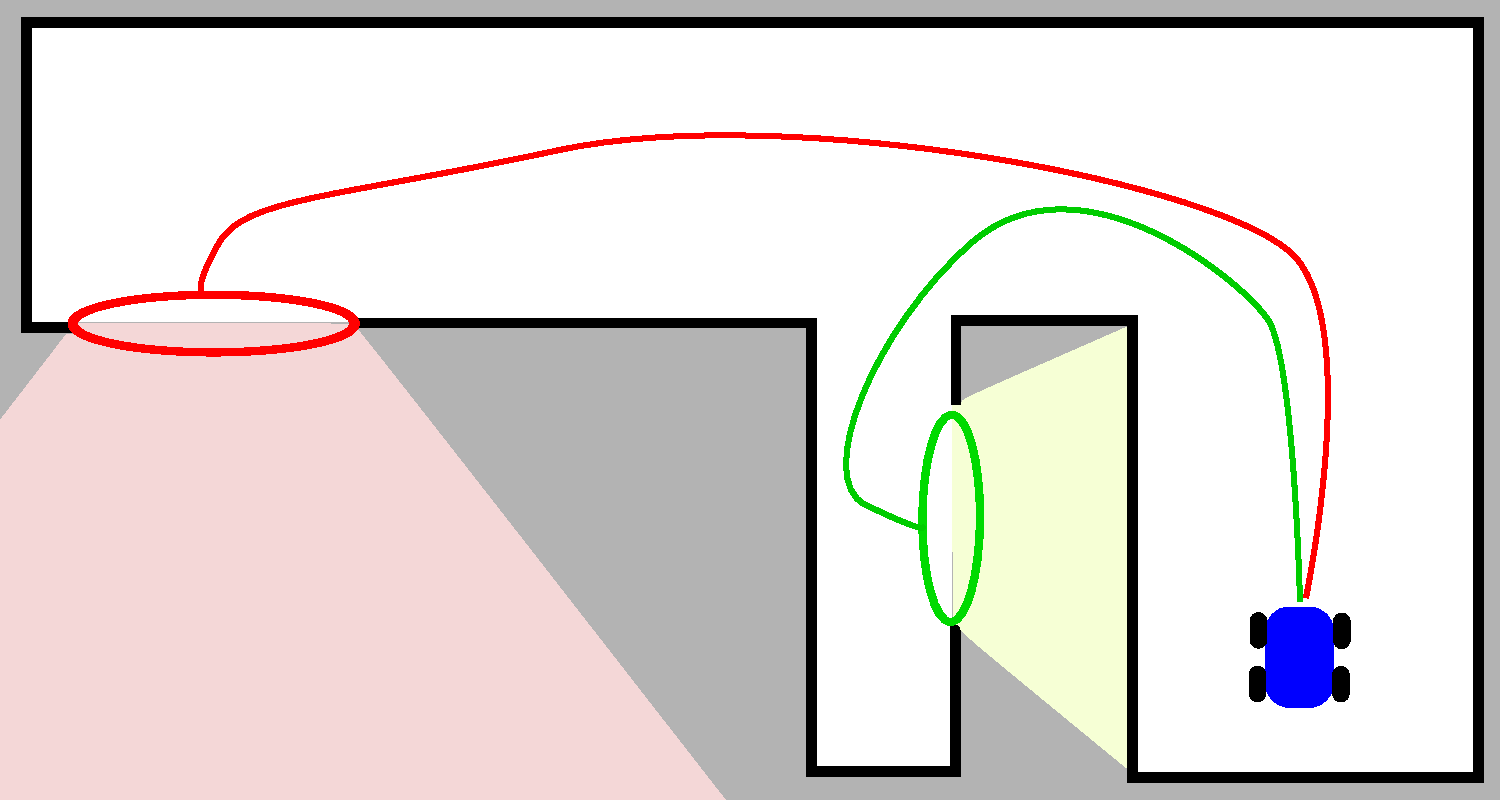
\includegraphics[width=0.7\textwidth]{sensor_frontier.pdf}
  \caption[Effects of modeling sensors on frontier exploration.]{Traditional frontier exploration would visit the green location first
    because it is closest. A simple extension involves simulating sensor
    measurements from frontiers and examining their informativeness~\cite{gonzalez2002navigation}. Applying this
    extension would cause robot to visit the red frontier first, since that
    location will provide more information about the map per unit time.\label{fig:sensor_frontier}}
\end{figure}

More thorough surveys of frontier exploration algorithms and heuristics are provided by
Basilico et al.~\cite{basilico2008evaluating} and Holz et al.~\cite{holz2011comparative}.

\subsection{Information-Theoretic Exploration Strategies}

Information-theoretic exploration strategies cast the active perception task as
an optimization, and choose actions for the robot that maximize an information-based objective function such
as Shannon's entropy or mutual
information~\cite{bourgault2002information,kollar2008efficient,charrow2015icra,julian2013mutual}
(Fig.~\ref{fig:mi_vs_csqmi}).
Entropic measures like these are appealing because unlike geometric methods,
they capture the relationship between sensor placement and uncertainty in the
map. In addition, they can be computed without a maximum likelihood map estimate, and
therefore do not discard probabilistic information known to the robot. Control policies
that maximize mutual information have been proven to guide robots
towards unexplored space~\cite{julian2013mutual}, and weighting frontiers by
the expected mutual information between the map and a sensor measurement
acquired at the frontier location has been shown to result in more efficient exploration
behaviors than traditional frontier exploration~\cite{charrow2015icra}.
The same calculation (involving raycasting along beams from a sensor
measurement) can be used to evaluate information-theoretic objective
functions in both 2D and 3D environments.

\begin{figure}[t]
    \centering
    \begin{subfigure}[t]{0.31\textwidth}
        \centering
        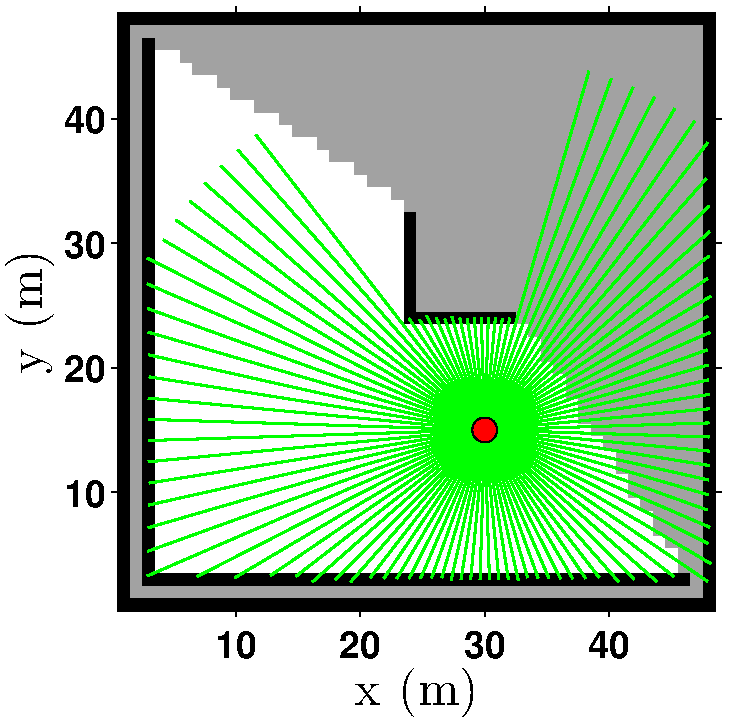
\includegraphics[height=4.0cm]{map.pdf}
        \caption{\label{fig:og}}
    \end{subfigure}
    \begin{subfigure}[t]{0.31\textwidth}
        \centering
        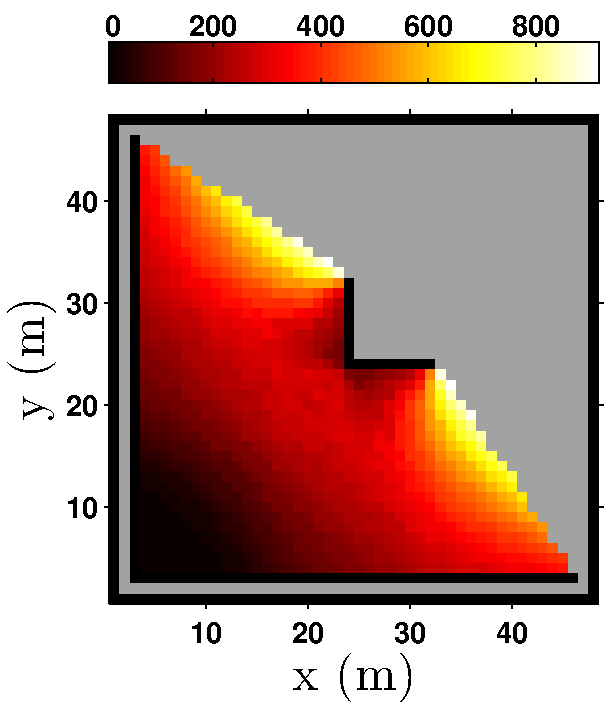
\includegraphics[height=5.0cm]{mi_map.pdf}
        \caption{\label{fig:og_mi}}
    \end{subfigure}
    \begin{subfigure}[t]{0.31\textwidth}
        \centering
        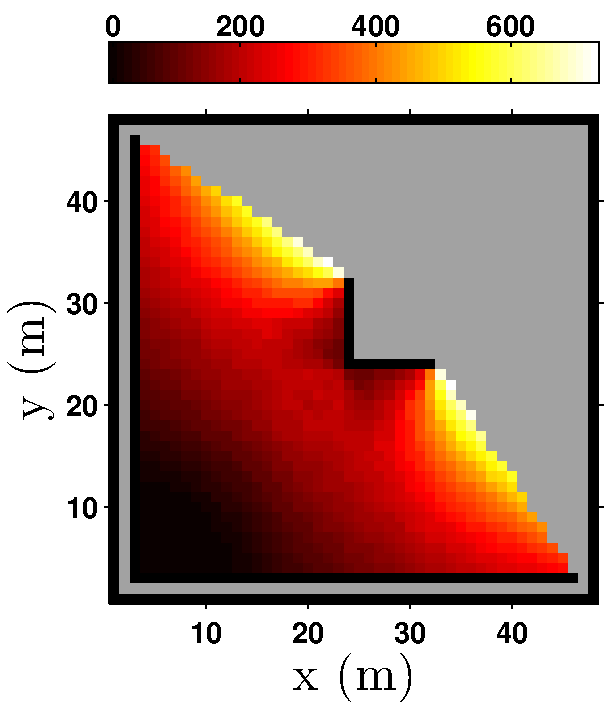
\includegraphics[height=5.0cm]{csqmi_map.pdf}
        \caption{\label{fig:og_csqmi}}
    \end{subfigure}
    \caption[Maximizing mutual information drives a robot to unexplored areas.]{Two variants of mutual information (Fig.~\ref{fig:og_mi}: Shannon;
    Fig.~\ref{fig:og_csqmi}: Cauchy-Schwarz Quadratic) densely computed in free space
  over an occupancy grid (Fig.~\ref{fig:og}) using a $100$-beam omnidirectional 2D
laser with $30$ m range. An exemplary sensor measurement is depicted in
Fig.~\ref{fig:og}. Controlling the robot towards locations that maximize either variant
of mutual information would attract the robot to locations from which it
could observe unknown areas of the map. \label{fig:mi_vs_csqmi}}
\end{figure}

The utility afforded by information-theoretic approaches comes at the cost of
computational inefficiency.
As a point of comparison, frontiers and other geometrically-defined landmarks
need only to be computed once per map update, and can be computed (at worst, using a brute force search)
with time complexity linear in the number of cells in the robot's map.
One may alternatively choose to identify and cache frontiers every time a sensor
measurement is used to update the map, yielding a constant time frontier
identification step that is bounded by the number of map voxels within the maximum sensor range.
By contrast, information-theoretic objective functions typically consider the probabilistic
uncertainty associated with the sensor and environment models, and therefore
require expensive sensor-related operations such as raycasts or sampling a large
number of times from the distribution of possible future measurements.
Approximations to mutual information between a map and beam-based sensor
measurements can be evaluated with time complexity linear in the number of map
voxels intersected by a sensor's
beams~\cite{julian2013mutualthesis,charrow2015icra,nelson2015iros}. This
already-expensive operation must be performed for every future location that the
robot might wish to travel to, or even multiple times along a single planned
action. Julian et al. report that densely calculating
mutual information over the free space in a large $1500$ m$^{2}$ map requires
approximately ten seconds with a parallelized implementation using a $3.4$ Ghz
quad-core CPU and NVIDIA GTX 690 graphics card~\cite{julian2013mutual}. While
impressive, these results demonstrate that dense evaluation of mutual
information over a robot's map is not feasible for high-speed applications that
require subsecond planning frequencies.

\section{Thesis Problem}
\label{sec:thesis_problem}

%Intuitively, the faster a robot travels, the more quickly it must evaluate the informativeness of
%locations that it could navigate towards in the future. With increasing speed,
%future actions that the robot may take become more fleeting; either they must be
%chosen immediately, or they must be discarded in favor of a different action.
%In other words, faster navigation requires higher planning frequencies, in turn
%demanding more calls to the subsystem handling {\bf component 1}.


This thesis focuses on the problem of enabling a mobile robot to
\textit{efficiently} explore its environment without human intervention.
A robot that explores efficiently will learn the largest map possible
for a fixed amount of time or energy input.
The robot is assumed to be initialized without a
priori access to a map, and is assumed to be capable of creating one in
real-time from incoming sensor measurements with a Simultaneous Localization and
Mapping (SLAM) subsystem~\cite{thrun2005probabilistic}. The robot's task is to select
control actions that maximize the likelihood that it will acquire informative sensor measurements
in the future, given that it only knows a partial representation of the
environment through which it is navigating. An \textit{informative sensor measurement}
is one that reduces uncertainty in the robot's map, allowing it to make
more informed subsequent decisions. The exploration task is
challenging because determining actions that will result in a minimum-time or
minimum-energy traversal of the environment is impossible (or highly unlikely) without
full a priori knowledge of the map. Instead, the environment must be modeled as a random
quantity whose structure is only understood after it is observed by the robot's
sensors.

State-of-the-art solutions to the exploration problem involve choosing control actions
that drive the robot to states from which it will receive sensor measurements that
maximally reduce uncertainty in its map (i.e. maximize an \textit{information-theoretic
reward function}). Although computationally
inefficient, this category of solutions drives a robot to unexplored territories
in a smaller amount of time than geometric exploration
approaches~\cite{charrow2015icra}. However, as evidenced by the infeasibility of
dense information-theoretic reward evaluation, there
remains room for improvement. For example, a highly-efficient recent approach by
Charrow et al. requires eleven minutes to explore a $17$ m $\times 18$ m $\times
3$ m building with a quadrotor - enough time for the robot's batteries to
deplete twice~\cite{charrow2015icra}. Any increase to the efficiency of
information-theoretic exploration will allow the robot to consider more future
actions before selecting and executing one. By considering more actions, a robot
might discover a highly informative location in the environment that it
previously would not have, increasing exploration performance.

This thesis addresses the computational costs of mobile robot exploration, summarized in the following statement:

%% Thesis Problem
\begin{center} \fbox{ \parbox{0.9\linewidth} { {\bf Thesis Problem:}
      The computational cost of exploration with a mobile robot scales with the robot's speed,
      environment complexity, and dynamic model complexity. Exploring at high
      speeds or in complex regimes therefore requires either increased computational
      resources, or methods to increase the efficiency of identifying and
      navigating to informative locations.
} } \end{center}

%\section{Thesis Statement}

%This thesis examines the relationship between a robot's environment
%representation and the efficiency of its exploration behaviors.
%Specifically, it considers compressing the robot's map to
%increase the speed at which information-theoretic reward can be computed along
%planned actions. \textit{Map compression} refers to the process of
%decreasing the map's resolution while retaining as much information as
%possible about obstacles and free space. Reducing the memory required to
%store the map necessarily causes structural information about the environment to
%be discarded. Compression therefore decreases the accuracy of information-gain
%computed with respect to a sensor measurement. The tradeoff between information accuracy and
%redundancy is investigated to characterize situations in which the robot's map may be
%compressed while sacrificing a minimal amount of information about an expected
%future sensor measurement. Reducing the amount of time required to evaluate
%reward over any one action allows the robot to consider more actions before
%its planning update rate forces it to choose one for execution.

%The idea of map compression, while primarily aimed to make exploration more
%efficient, opens the door to interesting new methods that can
%be used to analyze the complexity of the robot's environment. For example,
%as will be demonstrated in Chapter~\ref{chapter5},
%the information difference between an uncompressed and
%compressed map correlates with the obstacle-density of the environment.
%Therefore the same compression strategy can be used to persuade a robot to
%choose actions that are both informative and safe, avoiding obstacle-dense
%regions. This consideration also increases the speed of exploration; by
%implicitly avoiding obstacles, the robot will be drawn to open expanses where it
%need not be concerned about collisions, and will able to navigate more quickly.

%The ideas introduced in the remainder of this thesis culminate in the following
%statements:

%% Thesis Statement
%\begin{center} \fbox{ \parbox{0.9\linewidth} { {\bf Thesis Statement:} \\
%      %\begin{itemize}
%        %\setlength\itemsep{0.0em}
%      %  \item Compressing an occupancy grid map
%      %    increases the efficiency of computing information-theoretic reward
%      %    by orders of magnitude, thereby enabling faster planning and navigation during
%      %    exploration.
%      %  \item Maps can often be compressed in a way that minimally sacrifices the accuracy of
%      %    mutual information with respect to a sensor measurement.
%      %  \item Analyzing the loss in informativeness of sensor
%      %    measurements when compressing a map enables the robot to choose trajectories
%      %    that are both safe (avoiding obstacle-dense regions) and informative (maximizing
%      %    an information-theoretic reward).
%      %\end{itemize}
%} } \end{center}

%  \item Compressing the robot's map, when possible, increases the
%    efficiency of computing information-theoretic reward by orders of magnitude, thereby
%    enabling faster planning and navigation during exploration
%  \item Analyzing the loss in informativeness of sensor measurements when
%    compressing the map enables the robot to choose trajectories are both safe
%    (avoiding obstacle-dense regions)
%    and informative (maximizing an information-based reward).

\section{Contributions and Outline}

%The remaining chapters examine the relationship between a robot's environment
%representation and the efficiency of its exploration behaviors.
The thesis problem in Section~\ref{sec:thesis_problem} is addressed by
developing methods to increase the efficiency of identifying and ranking
the informativeness of future actions that the robot can take ({\bf component
1} of the active perception task). Map compression is proposed as a means of reducing the cost of evaluating information-theoretic
reward along planned actions. Map compression refers to the process of
decreasing the map's resolution while retaining as much information as
possible about obstacles and free space. Unfortunately, reducing the memory required to
store the map necessarily causes structural information about the environment to
be discarded (referred to as \textit{distortion}). Compression therefore decreases the accuracy of information-gain
computed with respect to a sensor measurement. The tradeoff between information accuracy and
redundancy is investigated to characterize situations in which the robot's map may be
compressed while sacrificing a minimal amount of information about an expected
future sensor measurement.

The structure of this thesis follows. Chapter~\ref{chapter2} provides an
overview of occupancy grid mapping, active perception, several planning
strategies, and foundational elements from information theory. These ideas will
be used to rigorously define the active perception problem and exact aspects of
it which are the most computationally inefficient. Chapter~\ref{chapter3}
develops a strategy for compressing an occupancy grid map to a lower resolution
using ideas from rate distortion theory. Since the compression strategy
in Chapter~\ref{chapter3} does not depend on the robot's sensor model,
information-theoretic rewards computed on a compressed map will necessarily
be distorted from those computed on an uncompressed map. Chapter~\ref{chapter4}
introduces an optimization to maximize compression for efficiency while
simultaneously minimizing sensing distortion.
Concluding remarks and avenues of future research are provided in Chapter~\ref{chapter5}.

%Reducing the amount of time required to evaluate
%reward over any one action allows the robot to consider more actions before
%its planning update rate forces it to choose one for execution.
